\documentclass[12pt,conference]{IEEEtran}
\usepackage{mathtools}

\usepackage{algorithm}% http://ctan.org/pkg/algorithms
\usepackage{algpseudocode}% http://ctan.org/pkg/algorithmicx

\usepackage{graphicx}
%\usepackage{textcomp}
\graphicspath{ {images/} }

\hyphenation{op-tical net-works semi-conduc-tor}

\begin{document}
\raggedbottom

\title{Improving the Accuracy of a Sequential Mining Model for Hurricane Trajectory Prediction}

\author{\IEEEauthorblockN{Jasmin Bissonnette, Caden Marofke, Taylor Cox}
\IEEEauthorblockA{Department of Computer Science\\
University of Manitoba\\
Winnipeg, Manitoba\\
Email: \{bissonnj, marofkec, coxt3\}@myumanitoba.ca}}

\maketitle

\begin{abstract}

In the 21st century alone, hurricanes have caused billions of dollars worth of damage due to property destruction, personal danger, and civil unrest. The catastrophic impact of hurricanes and other tropical storms has motivated extensive research into hurricane forecasting. Hurricane trajectory prediction is a subfield of hurricane forecasting that traditionally uses meteorological analysis to determine the future path of a given hurricane. While meteorological methods of hurricane trajectory prediction have been effective in the past, little attention has been paid to hurricane trajectory prediction with respect to historical frequent pattern mining. In this work, we propose multiple dimensions for improving the accuracy of data mining-based hurricane trajectory prediction. We propose the use of Haversine distance, a real-world distance formula for improved hurricane pattern matching accuracy. We also propose the use of weighted data to favor recent hurricane trends when training the trajectory prediction model. Finally, we use training data exclusively from the years 1950 to 2000 to reduce the impact of historical inaccuracies in hurricane recording methodologies. After implementing all three improvement dimensions on a contemporary data mining model for hurricane trajectory prediction based on AprioriAll, results show a prediction-correctness ratio 10.22\% higher than the current state-of-the-art, at 75.22\%.

\end{abstract}

\begin{IEEEkeywords}
Hurricane Trajectory, AprioriAll, Prediction, Pattern Matching
\end{IEEEkeywords}

\IEEEpeerreviewmaketitle

\section{Introduction}

Hurricanes are a specific type of tropical cyclone exclusive to the Atlantic basin \cite{def-hurricane}. Hurricanes are divided into five categories according the Saffir-Simpson scale, based on wind-speed and expected damage \cite{hurricane-cat}. In the United States alone, hurricanes incur damages valued as high as \$157BN \cite{hurricane-cost}. The damages incurred by hurricanes do not only include property damage, but also personal danger and in some cases widespread civil unrest \cite{hurricane-cost-non-financial}. These damages motivate extensive research in the field of hurricane prediction analysis. Hurricane prediction analysis is traditionally divided into the subfields of hurricane intensity prediction and hurricane trajectory prediction. This paper focuses exclusively on the subfield of hurricane trajectory prediction. In particular, the goal of this paper is to investigate and improve on the existing-state-of-the art in hurricane trajectory prediction systems based on sequential data mining.

Data mining is the nontrivial extraction of implicit, previously unknown, and potentially useful information from data \cite{data mining-def}. Data mining applies to an extremely wide range of applications, including clickstream mining, social network community detection, and artificial intelligence. The data mining subdiscipline of particular interest in this work is \textit{sequential} data mining. Sequential data mining uses a database of chronologically ordered inputs to mine frequent patterns and interesting association rules. These association rules are used to make predictions on future data entries such as future customer transactions. More specifically, association rules generated by sequential data mining algorithms including AprioriAll, SPIRIT and PrefixSpan can be used in the field of hurricane trajectory prediction. 

To the knowledge of the authors, the existing standard in hurricane trajectory prediction via data mining is developed by Dong et al in \cite{major-hurricane-model}. The work cited proposes a hurricane trajectory prediction model based on data mining (HTPDM) that uses a modified variant of AprioriAll, a common sequential mining algorithm \cite{AprioriAll-original}. HTPDM executes AprioriAll against historical hurricane trajectories from 1900 to 2000 to generate interesting trajectory association rules. These association rules are compared against test data composed of hurricane trajectories from 2001 to 2008. HTPDM divides a given testing trajectory into two parts: the initial trajectory $T_{i}$ and the terminal trajectory $T_{t}$. $T_{i}$ is compared against all association rule antecedents until a sufficiently matching rule R is found based on a predetermined fitness function. The consequent of R is then compared against $T_{t}$ using pattern-matching techniques to determine if the prediction was correct. The results of HTPM showed that the model was able to achieve a best-case correctness ratio of 65\%. In this work, HTPDM will be developed and various strategies will be employed to improve the correctness ratio. Reducing the impact of historical factors, favoring the impact of recent trends, and improving the realistic nature of the hurricane trajectory prediction model result in a new model dubbed WARD-HTP (Weighted-Asset, Realistic-Distance Hurricane Trajectory Predictor). The strategies employed in WARD-HTP ultimately result in a correctness ratio of 75.22\%, a 10.22\% improvement over HTPDM.

The remainder of this paper is structured as follows: First, Section II gives a detailed survey of related work in the hurricane prediction and sequential mining disciplines. Next, section III will cover the general motivations of this work with respect to hurricane trajectory prediction, and the specific motivations of this work with respect to improving the current state-of-the-art. Section IV will provide a description of the problem space, which includes specific implementation considerations in hurricane trajectory prediction. Section V will give an exposition of the solutions proposed in WARD-HTP for increasing the correctness ratio in hurricane trajetory prediction. Following that, Section VI will detail the experimental setup, including the training data and other experimental variables. Section VII will evaluate the results of the experiments, which show that the ideal configurations of WARD-HTP result in a maximal correctness ratio of 75.22\%. This work will then conclude with section VIII, capturing the conclusions and directions of future work.

\section{Related Work}

The development of an accurate hurricane trajectory prediction model is a problem which has received little attention in the data mining literature. Works including \cite{hurricane-intensity-1} and \cite{hurricane-intensity-2} have been completed to develop data-mining approaches to hurricane intensity prediction. These works however do not describe approaches to hurricane trajectory prediction. Hurricane trajectory prediction has been covered in previous meteorological and geographic information system (GIS) works. These types of hurricane trajectory forecasting models include those seen in \cite{hurricane-forecasting-1} or \cite{hurricane-forecasting-2}. The intersection between data mining and hurricane trajectory prediction has been sparsely investigated in the literature. Publications such as \cite{typhoon-clustering} proposed a clustering-based model for typhoon track prediction based on specific characteristics of historical data. Typhoons are then clustered into groups depending on the general trajectory patterns they exhibit. While the described work provided novel results in typhoon track clustering, it is not clear if the proposed solution is able to predict the trajectories of new storms. Additionally, the clusters developed apply specific to typhoons, which are waterborne storms native to the east-pacific seaboard. Such storm patterns may not be applicable to patterns found in hurricanes, which are waterborne storms of the west-atlantic seaboard. For this reason, the proposed clustering patterns were not used in this work.

The primary baseline of this work is \cite{major-hurricane-model}, which uses a specific implementation of AprioriAll (first proposed in \cite{AprioriAll-original}) to determine frequent hurricane trajectory patterns. These trajectory patterns correspond to interesting trajectory association rules, which are used to train a prediction model. The implementation of AprioriAll used in \cite{major-hurricane-model} is also used as the foundational model for this work. AprioriAll transforms a transaction database into a \textit{customer} database, where each entry contains a customer and an ordered sequence of purchased items. The ordered sequence database is then mined for frequent ordered patterns, or frequent sequences. The modification of Apriori proposed in \cite{major-hurricane-model} mines frequent ordered patterns and thus skips the transformation step of AprioriAll. 

The model proposed in this work uses historical hurricane trajectory readings from HURDAT, the canonical hurricane database maintained by the National Hurricane Center \cite{HURDAT2-original}. The data in HURDAT2 is ordered into $\langle Hurricane, Trajectory \rangle$ pairs, omitting the need for the sequence mapping step required at initialization of AprioriAll. The Atlantic hurricane trajectories recorded in HURDAT2 span a very large distance, some of which reaching over 10,000 kilometers in total distance travelled. As a result, the coordinates recorded are limited to those within a range of 0 to 50 degrees north, and 20 to 100 degrees west. This degree range is approximately the size of the south Atlantic basin.

% We might want some more related work

\section{Motivation}

There are two categories of motivation behind this work. The first motivation of this work is to increase the total investigation completed in the hurricane trajectory prediction subdiscipline. Little research effort has been allocated to this particular problem space of high economic, and social impact. The authors expect this work to constitute a growing effort by academic and government researchers to improve existing methods of hurricane trajectory prediction in the interest of public safety and economic stability.

The second motivation behind this work is the specific goal of improving the correctness ratio in the current standard data mining model for hurricane trajectory prediction. As previously described, HTPDM had a best case trajectory prediction correctness ratio of 65\%. This means that of all testing trajectory for a which a matching rule was successfully produced, 65\% of such matches were correct predictions. When HTPDM accounts for testing trajectories for which no rule could be matched, the correctness ratio decreases by 7.5\% to a final value of 57.5\% correctness. This decrease in accuracy is expected as some hurricane trajectories are outliers which cannot be predicted by frequent pattern mining, as will be discussed further in this work.

The motivation of improving the correctness ratio in the model encompasses the challenges of improving the best-case correctness ratio (the correctness ratio when ignoring rule-miss incidents) and the worst-case correctness ratio (the correctness ratio when accounting for rule-miss incidents). To resolve the motivations of this work, a series of improvement strategies are proposed as applications to the current hurricane trajectory prediction model based on AprioriAll. In general, these strategies seek to improve the realism of the prediction model, reduce historical factors which may negatively affect the model's correctness reatio, and favor recent hurricane trajectory trends which are likely to be reflected in current and future hurricane patterns.

\section{Problem Description}

% What are the things to know about the problem?
% - Algorithm: AprioriAll ( pseudocode )
% - hit rate/miss rate
% - regions ( show diagram )
% - define accuracy, rule fit, fitness function.. ( equations )

In this section, the problem of achieving accurate hurricane trajectory prediction is explained in detail. This problem consists of multiple challenges which apply generally to sequential data mining, and specifically to the problem domain of hurricane location analysis. Many of the domain-specific challenges of hurricane trajectory prediction arise from the fact that hurricane points are tracked as a series of $\langle Latitude, Longtitude \rangle$ points, which do \textit{not} directly correspond to traditional (x, y) coordinates, as latitude and longtitude are points imposed upon a sphere. Challenges including accurate distance evaluation are results of the transition from a Euclidean to a Polar coordinate system.

The exposition of the hurricane prediction problem domain is divided into three parts. The first aspect of the problem domain concerns the underlying sequential mining approach used. This includes a thorough description of AprioriAll, its intended usage, and the reaction of AprioriAll to its input parameters. Next, the subproblem of region discretization will be discussed. Since $\langle Latitude, Longtitude \rangle$ points constitute continuous space, hurricane trajectories are converted to sequences of discrete regions to enable the discovery of frequent patterns. Finally, problems involving hurricane trajectory matching will be discussed. These problems include pattern matching for determining best fit rules and pattern matching for determining trajectory prediction correctness.

\subsection{AprioriAll}

In HTPDM and WARD-HTP, the algorithm that generates trajectory prediction possibilities is based on AprioriAll. AprioriAll was first proposed at IBM research as a method for discovering frequent sequential patterns in transactional databases \cite{AprioriAll-original}. In its original implementation, AprioriAll is able to generate assocation rules describing sentences of the form ``Customers who buy P may also buy Q''. In the hurricane trajectory prediction problem, AprioriAll is used to generate association ruls describing sentences of the form ``Hurricanes located at P may later be located at Q''. In the context of AprioriAll, hurricanes are considered $customers$ and their sequences of recorded points are considered $transactions$. Consider the high-level implementation steps of AprioriAll as follows:

\begin{enumerate}
\item Map the transaction database into a customer database.
\item Generate frequent sequences based on minimum support.
\item Generate association rules based on minimum confidence.
\end{enumerate}

\subsubsection{Mapping}

In step (1) of AprioriAll, a given transaction database \textit{D} is grouped by customers, and the frequent items purchased by customers in individual transcations are recorded in a temporary table. The contents of this temporary table are mapped to corresponding sequences to enable the mining of frequent transaction sequences from the original database. The intention of step (1) is to map \textit{D} in its original $\langle TransactionID, CustomerID, Items\rangle$ database form into a database \textit{D'} of the form $\langle CustomerID, ItemSequence\rangle$. 

The hurricane trajectory model in this work does not implement step (1), as the training data from HURDAT2 was instead translated into a $\langle HurricaneID, CoordinateSequence\rangle$ database as a preprocessing step before any aspects of the model are executed. By directly translating the data instead of processing it with AprioriAll, all trajectories in the original database are preserved. This includes coordinates which may ultimately be infrequent. The sequential mapping of AprioriAll is performed as a preprocessing step so that the database used in the prediction model will always consist of hurricanes and their coordinate sequences. This allows the prepared (mapped) database to be mined directly without the need to complete the mapping step every time AprioriAll is executed.

\begin{figure}[ht]
\caption{Sample of mapped Hurricane-Coordinates database}
\centering
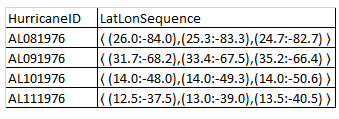
\includegraphics[scale=1.0]{hurricane-table-sample}
\end{figure}

Figure (1) shows an example of how the trajectory database is structured after the mapping preprocessing step. Only two dimensions are needed in the database, being the hurricane ID and the sequence of latitude-longtitude coordinates. All hurricanes in HURDAT2 have an ID corresponding to the location (the Atlantic), the index ordered by appearance in the hurricane year, and the year itself. For example, hurricane Katrina of 2005 corresponds to AL122005. The preprocessing step proposed is executed exactly once, allowing the hurricane database to be mined without the initial grouping and mapping stage.

\subsubsection{Sequence Generation}

Section (2) of AprioriAll initiates the generation of frequent sequences. In the case of hurricane trajectory prediction, these sequences correspond to frequent recorded hurricane coordinate sequences. Frequent hurricane coordinate sequences are those which occur at least a minimum number of times, as defined by the \textit{minimum support}, or minsup. In general terms, the sequence generation step of AprioriAll develops frequent ordered patterns of increasing length, beginning with frequent single-item sequences (corresponding to frequent single-point sequences). This step begins by scanning the $\langle HurricaneID, CoordinateSequence\rangle$ database for frequent single-point sequences. The frequent single-point trajectories are then converted to candidate two-point trajectories as the result of an inner join. The candidate two-point trajectories are scanned against the database to determine which candidates satisfy the minimum support. Another inner join generates the candidate 3-length trajectories. Once the sequence generation level reaches three, each candidate sequence must be pruned if any of their candidate subsequences are infrequent. Continuous execution of AprioriAll until completion results in a collection of frequent hurricane trajectory patterns, as defined by the minumum support.

%AprioriAll Pseudocode
\begin{algorithm}[H]
  \caption{Modified AprioriAll: No Litemset phase}
  \label{aprioriall_for_hurricanes}
  \begin{algorithmic}[1]
  \State{$L_{1} \gets \{Frequent\ Single\ Points\}$}
  \For{($k=2; L_{k-1} \neq \emptyset k++)$}
    \State{$C_{k} \gets Candidates\ from\ Inner\ Join$}
    \State{$Prune\ C_{k}\ of\ infrequent\ subsequences\ $}
    \For{$sequence\ S \in HurricaneDB$}
      \State{$Increase\ c \in C_{k}\ support\ if\ c \in S$}
    \EndFor
    \State{$L_{k} \gets \{c \in C_{k}|\ sup(c) \geq minsup\}$}
  \EndFor
  \State{$Frequent Trajectories \gets All(L_{k})$}
  \end{algorithmic}
\end{algorithm}

Along with HTPDM, WARD-HTP executes AprioriAll with a slight modification to the existing algorithm proposed in \cite{AprioriAll-original}. Whereas L1, the frequent single-item sequences is generated by the L-Itemset (mapping) phase of AprioriAll, the variant of AprioriAll used in hurricane trajectory prediction skips the L-Itemset phase, and thus scans the $\langle HurricaneID, CoordinateSequence\rangle$ directly for frequent single-point trajectories. Otherwise, the remainder of AprioriAll is used in this work as originally designed. AprioriAll is used to ensure that the order of recorded hurricane coordinate sequences is preserved. This is a product of the inner-join step. Consider two hurricane trajectories $T_{1}$ and $T_{2}$. $T_{1}$ and $T_{2}$ form a new trajectory $T_{3}$ if and only if the \textit{L}-1 terminal coordinates of $T_{1}$ correspond to the \textit{L}-1 initial coordinates of $T_{2}$, where \textit{L} is the current level of AprioriAll being executed. For example, if \textit{L}=2, then AprioriAll scans for frequent 2-coordinate sequences, and uses those frequent 2-coordinate sequences to generate 3-coordinate sequences based on trajectory matching. If the matching condition is satisfied, a new trajectory is generated. The inner-join step of AprioriAll emulates the required hurricane trajectory-matching to develop frequent hurricane trajectory patterns. Once all possible frequent hurricane trajectory patterns are discovered, the second step of AprioriAll completes.

\subsubsection{Rule Generation}

The final step of AprioriAll is the rule-generation step. Though association rule generation is not a specific stage of the AprioriAll algorithm, it is traditionally the final stage of any association rule mining approach. The rule generation step is responsible for developing interesting association rules. As mentioned, rules generated by the hurricane trajectory prediction model proposed will satisfy sentences of the form ``Hurricanes located at P may later be located at Q''. 

Association rules are derived directly from frequent patterns generated by AprioriAll or any modified versions. These rules consist of four dimensions: the antecedent, consequent, support and confidence. An association rule \textit{R} is generated by partitioning a frequent sequence \textit{S} into two congruent parts. The left partition of \textit{S} constitutes the antecedent of \textit{R}, and the latter partition is the consequent. The support of \textit{R} is the original support of \textit{S}. The confidence of \textit{R} is the support of \textit{S} divided by the support of the subsequence given by the former partition. 

Rules with confidence of at least the \textit{minimum confidence} (minconf) are stored in a table of interesting association rules. The rules generated by AprioriAll are the candidates for hurricane trajectory pattern matching. Hurricane trajectories are matched against all association rule antecedents. The consequent of the closest match rule is then used to predict the hurricane terminal trajectory. If the association rule consequent matches the actual hurricane terminal trajectory, the prediction is considered correct. Without the association rules formed by AprioriAll and the rule generation step, data mining-based hurricane trajectory prediction cannot be executed. HTPDM and WARD-HTP both use historically frequent hurricane trajectory to predict the result of future hurricane paths.

\subsection{Region Discretization}

This subsection covers problems related to the discretization of $\langle Latitude, Longtitude \rangle$ points. As shown in figure (1), the raw recorded hurricane coordinates are expressed in degrees and minutes. The excessively fine-grained nature of the raw data prevents the data from being able to produce meaningful frequent coordinate sequences. Therefore, effort must be taken to discretize the coordinate system, allowing more coarse-grained frequent patterns to be produced.

In HTPDM and WARD-HTP, recorded hurricane coordinates are discretized into approximately square blocks of a specific size, expressed in degrees. Consider the first row of coordinates shown in figure (1): (12.5:-37.5), (13.0:-39.0), (13.5:-40.5). Mapping this coordinate sequence to a discritization block of size 5, the new trajectory becomes (2:-7), (2:-7), (2:-8). Duplicate coordinates are not counted, so the trajectory ultimately reduces to (2:-7), (2:-8). Note that the degree-size of the discretization block is expressed as an integer, which means that all coordinates are mapped to their lowest divisor relative to the discretization size. This enables the coarse-grained mapping of coordinates to their corresponding region block. 

% Figures 2 and 3: Trajectories without and with region overlay
\begin{figure}[htp]
\caption{Sample Hurricane Trajectory Paths}
\centering
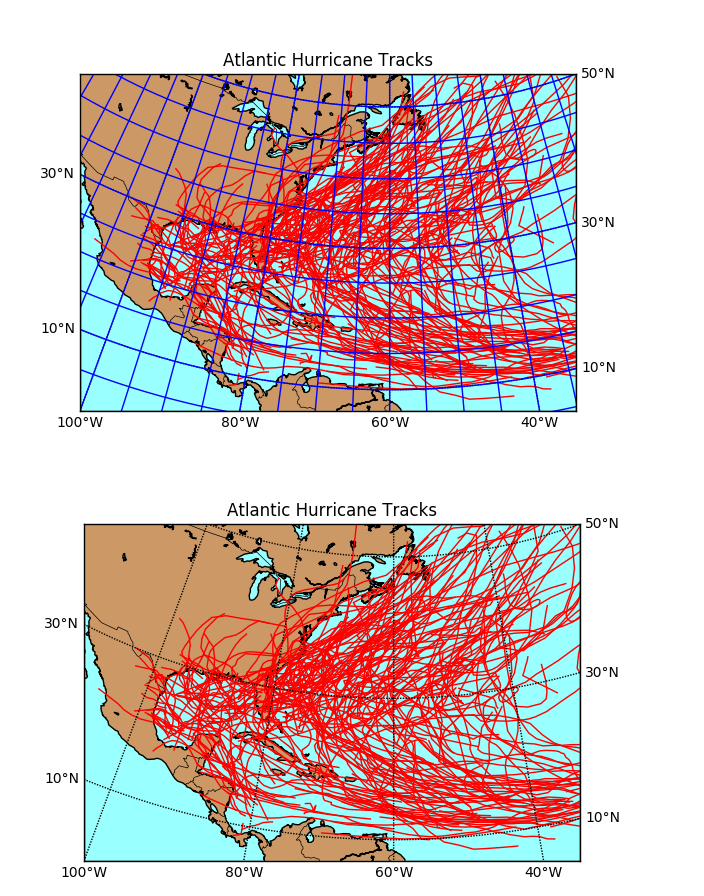
\includegraphics[scale=0.55]{Merged-Trajectory-Comparison}
\end{figure}

Consider figure (2), generated using a sample of the recrded hurricane trajectories in HURDAT2 with the visualization tool Matplotlib \cite{matplotlib}. As shown in the pair of images, region discretization organizes continuous hurricane coordinate sequences into discrete region sequences of approximately uniform size and square shape. A discretization block size of 5 is selected in HTPDM and is replicated in WARD-HTP. A block size of 5 corresponds approximately to a real-world block dimension of 500km by 500km. The block dimension size is approximate because the mapping between coordinate degrees and kilometers is imprecise, and is dependent on location in the case of longtitudal points \cite{lat-long-distance}. The approximate size of 500km is similar to the average hurricane total diameter \cite{hurricane-distances}, permitting the coarse-grain expression of hurricane trajectories without undue loss in precision.

All aspects of hurricane trajectory prediction with data mining depend on region discretization. Frequent trajectory patterns and their resulting trajectory predictions are expressed in terms of the regions where a given hurricane is expected to appear. The process of region discretization allows for hurricane coordinate trajectories to be scaled down, allowing the regionalized coordinates to be treated as a simplified coordinate system in subsequent aspects of the prediction model.

\subsection{Trajectory Matching}

The final key aspect of the hurricane trajectory prediction problem concerns accurate hurricane trajectory pattern matching. Pattern matching is a concern for hurricane trajectory prediction in two primary areas. First, hurricane trajectory matching must be effectively employed when comparing a new hurricane trajectory against the table of hurricane association rules generated by the previously described variant of AprioriAll. Hurricane trajectory matching is also used when checking the correctness of a trajectory prediction. The consequent of the matched hurricane trajectory rule is compared with the actual hurricane terminal trajectory to determine prediction correctness.

\subsubsection{Rule-Fit Matching}

Pattern matching is used when evaluating the best-fit rule for hurricane prediction purposes. Similar to HTPDM, a new hurricane trajectory is passed into the hurricane prediction model proposed in this work, it is separated into two subtrajectories: the initial trajectory $T_{i}$ and the terminal trajectory $T_{t}$. $T_{i}$ is compared against the antecedent of every interesting assocation rule satisfying minconf for a match. There are two dimensions that determine the best-fit rule for an incoming trajectory requiring prediction. These dimensions are matching length and rule confidence. The matching length of the initial trajectory $T_{i}$ to a rule antecedent is the longest congruent subsequence of regionalized points within the rule antecedent within $T_{i}$. Note that both $T_{i}$ and the rule antecedent sequences have been regionalized per the regionalization methodology outlined. Using the fitness function described in HTPDM \cite{major-hurricane-model}, the best-fit rule match for the incoming initial trajectory $T_{i}$ is expressed with the following formula:
\begin{eqnarray*}
Match = max( conf_{r} * (1 - e^{-matchLen_{t,r} } )\ ), r \in R
\end{eqnarray*}
Where r is a member of the set of all interesting assocation rules \textit{R}, t is the initial trajectory $T_{i}$, and $matchLen_{t,r}$ expresses the matching length between $T_{i}$ and the antecedent sequence of r. This formula is meant to be maximized to determine the rule which most generously fits the incoming hurricane trajectory. Once a best fit rule is determined, the rule consequent is compared with the \textit{actual} terminal hurricane trajectory to determine if the prediction is correct.

\subsubsection{Prediction Correctness Matching}

Prediction Correctness checking is also powered by hurricane trajectory pattern matching. The consequent of the best-fit rule generated by the rule-fit matching stage constitutes the predicted terminal sequence for the incoming hurricane trajectory. The best-fit consequent is then compared against the actual terminal trajectory $T_{t}$ to determine the prediction correctness. In HTPDM and WARD-HTP, prediction correctness is considered a binary attribute: a prediction is either correct or incorrect. If the matched-rule consequent also matches the incoming hurricane terminal trajectory, the prediction is correct and the model's correctness ratio is increased accordingly.

The pattern matching for rule consequents has some differences compared to antecedent pattern matching. First, prediction correctness uses matching length with a different definition. Whereas matching length for rule antecedents is the longest identical congruent subsequence of the initial trajectory, matching length for the rule consequent is the longest congurent subsequence of points within a specific distance, beginning at the start of the terminal sequence. This methodology is also based on HTPDM and is based on the following steps. In the algorithm given, $conseq_{r}$ corresponds to the matched rule's consequent sequence, and D corresponds to the minimum distance threshold necessary for prediction correctness. In HTPDM, the distance threshold corresponds to a Euclidean distance of 1.

\begin{algorithm}[H]
  \caption{Consequent Matching for Prediction Correctness}
  \label{consequent_matching}
  \begin{algorithmic}[1]
  \State{$l \gets min(|conseq_{r}|, |T_{t}|)$}
  \State{$Select\ first\ l\ points\ of\ conseq_{r}$}
  \State{$Select\ first\ l\ points\ of\ T_{t}$}
  \If{$All\ corresponding\ points\ within\ D$}
    \State{$Prediction:\ CORRECT$}
  \EndIf
  \end{algorithmic}
\end{algorithm}

The hurricane trajecory prediction model based on data mining as originally proposed in \cite{major-hurricane-model} implements all aspects of the problem domain described. Modified AprioriAll, downscaled region discretization and pattern matching with respect to association rule antecedents and consequents are respectively employed by HTPDM in order to develop an effective system for predicting future hurricane trajectories. Based on Atlantic hurricane trajectory data from 1900 to 2008, the model generates a best-case correctness ratio of 65\% and a worst-case ratio of 57.5\%. The training data used in the original model consists of trajectories from 1900 to 2000, with testing data supplied by trajectories from 2001 to 2008. At a high level, the model is developed and tested by following the steps below, using all implementation strategies discussed. 

% Model formal explanation could be better. Maybe do pseudocode

\begin{enumerate}
\item Generate interesting trajectory rules from AprioriAll
\item Determine matching rule for incoming trajectory 
\item Check if the matched rule's consequent points are sufficiently close
\end{enumerate}

The differentiation between the model's best and worst-case hit rates is dependent on the ability of an incoming test trajectory to be matched with a trajectory association rule. As described in the pattern matching stage, the initial subtrajectory of an incoming trajectory is compared against all interesting rules to determine a best-fit match. If no such match is found, HTPDM attempts to extrapolate a future point of the initial trajectory, using the extrapolated point as a new option for determing a rule antecedent match. When accounting for all tested trajectories, including those which were matched to a rule as a result of trajectory extrapolation, the correctness ratio was 57.5\%. Therefore, the best case correctness ratio of HTPDM is the ratio which ignores all test trajectories which did not match with any rules, resulting in a final value of 65\%.

Despite establishing a convincing initial start point, the best-case correctness ratio of 65\% may be too low for HTPDM to be considered realiable in the real-world. This is problematic for those interested in hurricane trajectory prediction as a model with only 65\% accuracy may not be able to deliver crucial insight into hurricane trajectory prediction, particularly with respect to landfall location prediction. Both correctness ratios given must be improved in order for data mining to be considered a reliable approach to predicting the trajectories of future hurricanes.

\section{Solution}

In order to improve the correctness ratio of datamining-based hurricane trajectory prediction, this work identifies and explores three opportunities for worst-case and best-case ratio improvement. The opportunities for improvement are the improvement of realism, reduction of historical impact, and favorability towards recent hurricane trends. Therefore, the opportunities for improvement are realized by three unique dimensions. These dimensions are the use of a distance formula designed for spherical coordinate systems, the Haversine Distance Formula, the use of weighted training data when executing the modified variant of AprioriAll, and the modification of the training data to only use historical trajectories from 1950 to 2000. The implementation of these three dimensions results in a new hurricane trajectory prediction model dubbed WARD-HTP (Weighted-Asset, Realistic-Distance Hurricane Trajectory Predictor). The combined contributions of WARD-HTP are expected to result in improvements to the best-case and worst-case correctness ratios.

\subsection{Haversine Distance Formula}

\subsection{Weighted Training Data}

\subsection{Training Data Year Interval}

\section{Experimental Setup}

\section{Experimental Results}

\section{Conclusions and Future Work} % what we found:

\begin{thebibliography}{1}
\bibitem{def-hurricane}  
\bibitem{hurricane-cat} 
\bibitem{hurricane-cost} 
\bibitem{hurricane-cost-non-financial} 
\bibitem{data mining-def} 
\bibitem{major-hurricane-model} 
\bibitem{HURDAT2-original} 
\bibitem{AprioriAll-original} 
\bibitem{hurricane-intensity-1}
\bibitem{hurricane-intensity-2}
\bibitem{hurricane-forecasting-1}
\bibitem{hurricane-forecasting-2}
\bibitem{typhoon-clustering}
\bibitem{matplotlib}
\bibitem{lat-long-distance}
\bibitem{hurricane-distances}

\end{thebibliography}

\end{document}

% there will be lots of editing %

% Early callouts:
% Motivation could be more clear
% We need to make sure we are explaining rule-miss incidents and our approach to them
% We also need to make sure we explain what exactly the correctness ratio is and how it changes based on accounting for rule-miss
% Also need to explicitly call out what our minconf was and why
% future work: non-binary prediction correctness?
% More non-text assets?
% We have done a good job describing the problem space but we need to explain what we problems __are__
% ie: why is there a solution
% we will need to re-read the paper and keep an eye out for sections that suffer from scope creep. Problem description first comes to mind.